It has been repeatedly shown that \ac{lora} transmissions can be received at distances exceeding 10km in  unobstructed environments (free-space) when antennas are highly elevated \cite{3YP:LORA_RANGE_REVIEW}. However, these ideal radio conditions are unrealistic for swarm robots operating close to the ground in high-propagation environments such as forests. Therefore the first experiment in this paper identifies \ac{lora}'s physical performance and scenario specific limitations. Due to expected sparsity, only far field scenarios are relevant ($d_{\text{SP}\leftrightarrow \text{MP}} >  0.35$m).


\section{Methodology}
The purpose of this testing was to inform protocol decisions and assess capability of an off-the-shelf \ac{lora} \ac{phy}. A focus was taken to get enough data across a small selection of important scenarios and parameters to allow quantitively assessment. 

 The two main transmission environments selected were free-space and in-forest; this was to give an understanding of both low-propagation and high-propagation scenarios. Data collection was mainly spread over two locations: \textbf{$L_{A}$} and \textbf{$L_{B}$} (split into \textbf{$L_{B1}$} and \textbf{$L_{B2}$}), identified in Figure \ref{fig:new_forest_map} and \ref{fig:stansted_map} respectively. All locations were rural and therefore theoretically free from strong sources of external interference. Radio placement was decided by first placing the transmitting radio (slave) at a fixed location (\ac{sp}), and then, using the furthest receivable point as the starting point for the receiving radio (master). From there the master was positioned closer towards the slave for each future test (\ac{mp}). In each scenario the main interest was ground level transmissions; however, to assess whether radio performance was actually compromised by the placement, comparative measurements were taken with an elevated antenna. 
 
  \begin{figure}[H]
    \centering
    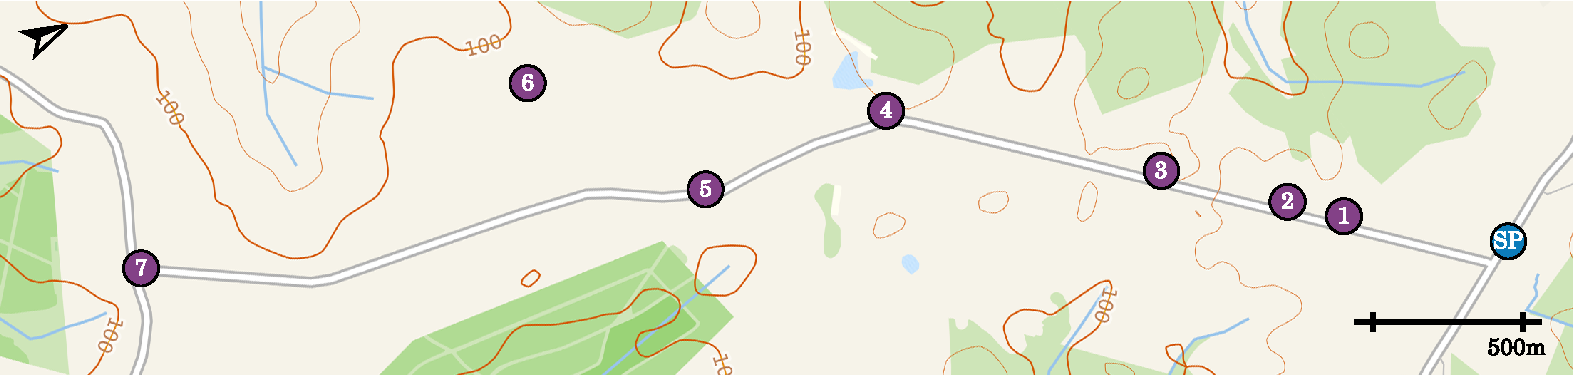
\includegraphics[width=\textwidth]{Figures/new_forest_light}
    \caption[Test Location: The New Forest, Hampshire, UK]{
    Test positions for \textbf{$L_A$} :  The New Forest, Hampshire, UK.\protect\footnotemark[1] \\
    \ac{sp} in open with \ac{los} to other points a combination of free-space and light vegetation. Exact positions are in Appendix \ref{sec:new_forest_test_pos}. To the left of \ac{mp}7 vegetation density increases,  making \ac{mp}7 the furthest position viable for free-space testing.
    }
    \label{fig:new_forest_map}
\end{figure}

\begingroup
 \begin{figure}[H]
    \centering
    \begin{tabular}{c}
    \subfloat[{
    Test positions for in-forest testing (\textbf{$L_{B1}$}). \ac{sp} in forest with \ac{los} to other points continually obstructed by a combination of leaved and bare trees. Exact positions are in Appendix \ref{sec:stansted_forest_test_pos}. Large clump of \ac{mp}s where radio reception was inconsistent.
    }]
    {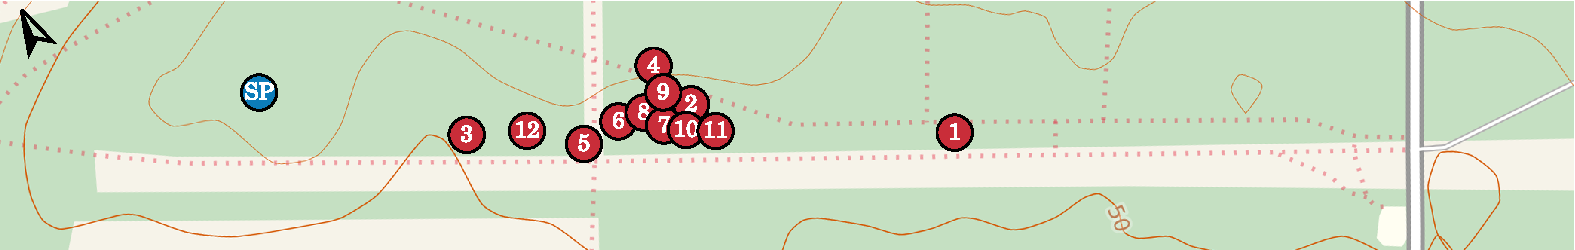
\includegraphics[width=\textwidth]{Figures/stansted_forest}\label{fig:stansted_map_forest}} 
    \\
    \subfloat[{
        Test positions for free-space testing (\textbf{$L_{B2}$}). \ac{sp} in open with \ac{los} completely free-space. Exact positions are in Appendix \ref{sec:stansted_free_test_pos}. No access to right of \ac{mp}13.
    }]{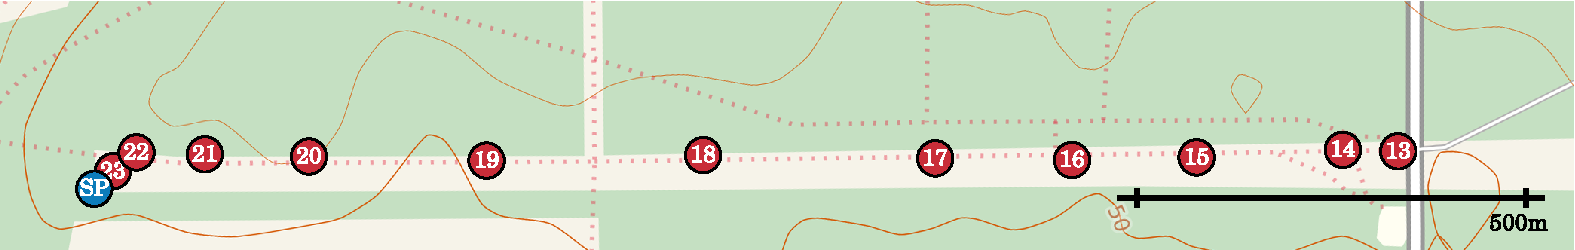
\includegraphics[width=\textwidth]{Figures/stansted_free_space}\label{fig:stansted_map_free}}
    \end{tabular}
    \caption[Test Location: Stansted Forest, West Sussex, UK]{
    Test locations for \textbf{$L_B$} :  Stansted Forest, West Sussex, UK.\footnotemark[1]
    }
    \label{fig:stansted_map}
\end{figure}
\footnotetext[1]{
    	$\enskip $ Copyright © 2019 MapOSMatic/OCitySMap developers\\
    	\indent \indent $\enskip $ Map Data © 2019 OpenStreetMap contributors (see http://osm.org/copyright)\\
    	\indent \indent $\enskip $ British Style © MapQuest \\
    	\indent \indent $\enskip $ Contour Overlay © OpenSnowMap.org
}

 In terms of radio parameters, \ac{sf} was the main focus due to it being an on option mostly unique to \ac{lora}; all values were tested for this in all locations ($\text{\ac{sf}} = 7, 8, 9, 10$). Variations using the lowest (4/5) and highest (4/8) \ac{cr}s were collected to verify \ac{fec} performance. Additionally, as the maximum transmission unit is often defined by the protocol, the effects of varying packet length were taken (\ac{pl} = 20, 128, 255 [\ac{phy} limit]). The rest of the parameters were fixed. The 868.1MHz \ac{cf} was used with \ac{tp} set to 14dBm so that collected data would be relevant in regard to \ac{etsi} regulations. The bandwidth was fixed to 125kHz so that radio sensitivity was only affected by the \ac{sf}. The \ac{ps}s were set to 8 to match \ac{lorawan} \cite{3YP:LORAWAN_REGIONAL_PARAMS}. The number of packets (\ac{pc}) transmitted for each configuration was set to 50; though not guaranteed, this gave reasonable expectation of a normal distribution. See Table \ref{tab:TestDefinitions} for full test definitions.
 
 To test the point-to-point transmissions, two identical platforms, which together could log the performance of sending and receiving \ac{lora} transmissions, were required. The platforms had to be suitable for outdoor use, be able to test multiple radio configurations whilst on location and provide a mechanism to indicate to user when the maximum range had been reached. The hardware and corresponding software created for this purpose is detailed in Appendix \ref{sec:testing_platform}.
\begin{figure}[H]
    \centering
    \begin{tabular}{ccc}
    \subfloat[][$L_{A}$ : MP05 \\ (1.0m)]{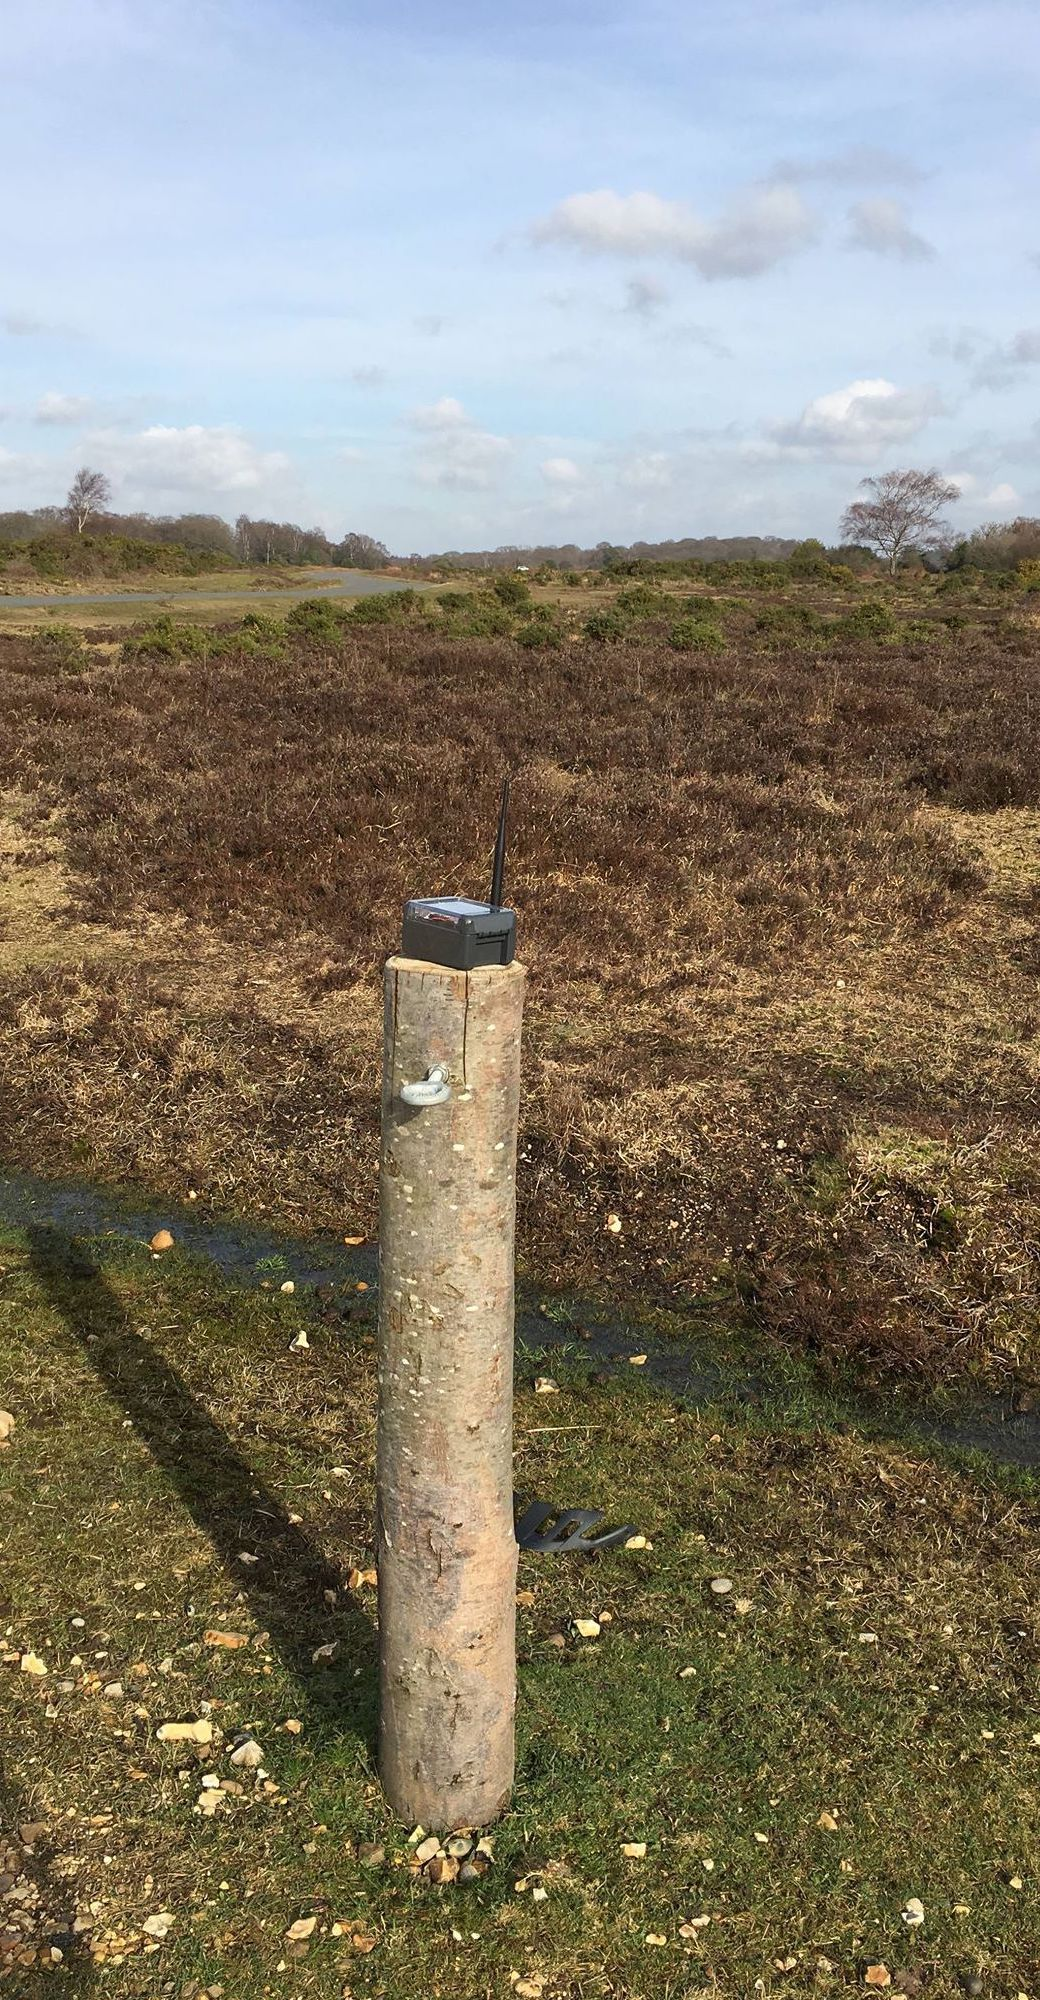
\includegraphics[height=7.5cm]{Figures/la_MP5_H1_0}}
    \hspace{2.5mm}
    \subfloat[][$L_{B1}$ : SP \\ (0.5m)]{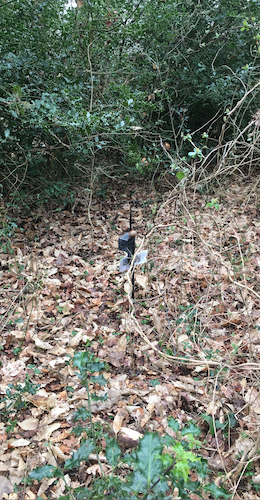
\includegraphics[height=7.5cm]{Figures/lb1_SP_H0_5}}
    \hspace{2.5mm}
    \subfloat[][$L_{B2}$ : MP16 \\ (0.0m)]{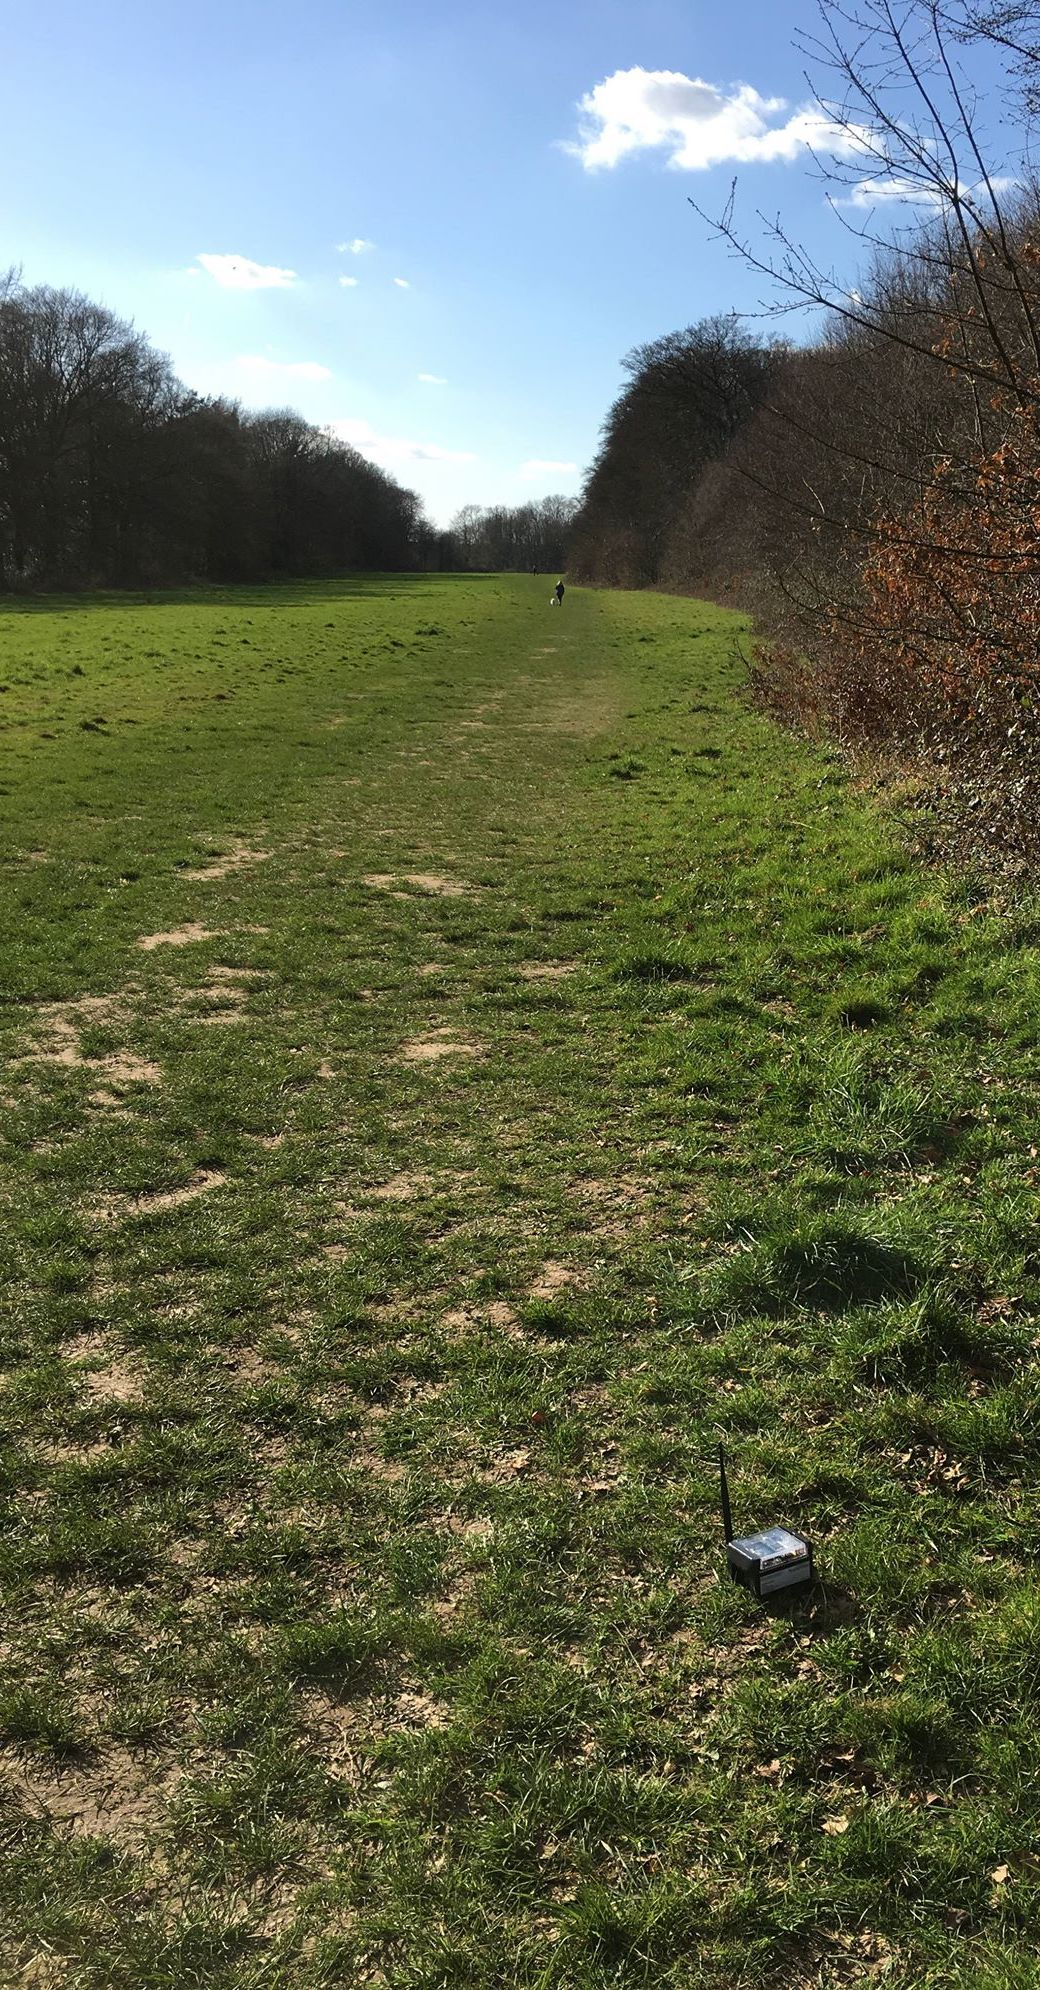
\includegraphics[height=7.5cm]{Figures/lb2_MP16_H0_0}}
    \end{tabular}
    \caption[Test location example]{Pictures of test environments and conditions. Although testing was split across multiple days at each location, the same dry conditions were present.}
    \label{fig:dataloggers}
\end{figure}
\endgroup
\vspace*{\fill}


 